\documentclass[aspectratio=169,xcolor=dvipsnames]{beamer}
\usetheme{Madrid}\usecolortheme{seahorse}
\usepackage{amsmath,amssymb,listings,tikz,booktabs,hyperref}
\lstset{language=Python,basicstyle=\small\ttfamily,keywordstyle=\color{blue}\bfseries,
  commentstyle=\color{OliveGreen},stringstyle=\color{red},frame=single,breaklines=true}

\title[Algorithms -- Week 2]{\textbf{Thiết kế và Phân tích Thuật toán}\\
  \large Week 2: Asymptotic Notation \& Complexity Classes}
\subtitle{TOAE209/TOAH209 -- Foreign Trade University}
\author{Department of Technology \& Data Science}
\date{Semester 2024--2025}
\AtBeginSection[]{\begin{frame}<beamer>{Outline}\tableofcontents[currentsection]\end{frame}}

\begin{document}
\begin{frame}\titlepage\end{frame}
\begin{frame}{Outline}\tableofcontents\end{frame}

\section{Motivation}
\begin{frame}{Why Formal Notation?}
  \begin{itemize}
    \item Saying "Algorithm A takes $3n^2 + 5n + 2$ operations" is implementation-specific
    \item We want to compare algorithms \textbf{machine-independently}
    \item Asymptotic notation captures the \textbf{essential growth rate}
    \item It lets us ignore constant factors and lower-order terms
  \end{itemize}
  \begin{exampleblock}{Intuition}
    For large $n$: $1000n < n^2/1000$ when $n > 10^6$.\\
    The algorithm that looks slower for small $n$ may dominate for large $n$.
  \end{exampleblock}
\end{frame}

\section{Big-O, Big-Omega, Big-Theta}
\begin{frame}{Formal Definitions}
  \begin{block}{Big-O (Upper Bound)}
    $f(n) = O(g(n))$ iff $\exists\, c > 0,\, n_0 > 0$ such that
    $0 \le f(n) \le c \cdot g(n)$ for all $n \ge n_0$.
  \end{block}
  \begin{block}{Big-Omega (Lower Bound)}
    $f(n) = \Omega(g(n))$ iff $\exists\, c > 0,\, n_0 > 0$ such that
    $0 \le c \cdot g(n) \le f(n)$ for all $n \ge n_0$.
  \end{block}
  \begin{exampleblock}{Big-Theta (Tight Bound)}
    $f(n) = \Theta(g(n))$ iff $f(n) = O(g(n))$ AND $f(n) = \Omega(g(n))$.\\
    Equivalently: $\exists\, c_1, c_2 > 0,\, n_0$ such that
    $c_1 g(n) \le f(n) \le c_2 g(n)$ for all $n \ge n_0$.
  \end{exampleblock}
\end{frame}

\begin{frame}{Worked Examples}
  \textbf{Prove:} $2n^2 + 3n + 1 = \Theta(n^2)$
  \begin{enumerate}
    \item \textbf{Upper bound ($O$):} $2n^2 + 3n + 1 \le 2n^2 + 3n^2 + n^2 = 6n^2$ for $n \ge 1$. Take $c_2 = 6$.
    \item \textbf{Lower bound ($\Omega$):} $2n^2 + 3n + 1 \ge 2n^2$ for $n \ge 0$. Take $c_1 = 2$.
    \item Thus $2n^2 \le 2n^2 + 3n + 1 \le 6n^2$ for $n \ge 1$. \hfill $\square$
  \end{enumerate}
  \vspace{0.5em}
  \textbf{Common mistakes:}
  \begin{itemize}
    \item $O(n^2)$ does \emph{not} mean "exactly $n^2$" — it's an \emph{upper bound}
    \item $2n = O(n^2)$ is \emph{true} but not tight
    \item We say "$f(n)$ \emph{is} $O(g(n))$" not "$f(n)$ \emph{equals} O(g(n))$" (technically)
  \end{itemize}
\end{frame}

\begin{frame}{Little-o and Little-omega}
  \begin{block}{Little-o (Strict Upper Bound)}
    $f(n) = o(g(n))$ iff $\lim_{n\to\infty} \frac{f(n)}{g(n)} = 0$.\\
    \textit{$f$ grows strictly slower than $g$}
  \end{block}
  \begin{block}{Little-omega (Strict Lower Bound)}
    $f(n) = \omega(g(n))$ iff $\lim_{n\to\infty} \frac{f(n)}{g(n)} = \infty$.
  \end{block}
  \vspace{0.3em}
  \textbf{Examples:}
  \begin{itemize}
    \item $n = o(n^2)$: $\lim n/n^2 = \lim 1/n = 0$ \checkmark
    \item $n^2 = \omega(n\log n)$: $\lim n^2/(n\log n) = \lim n/\log n = \infty$ \checkmark
    \item $n\log n \ne o(n^2)$? Actually it IS: $\lim \frac{n\log n}{n^2} = \lim \frac{\log n}{n} = 0$
  \end{itemize}
\end{frame}

\begin{frame}{Properties of Asymptotic Notation}
  \begin{itemize}
    \item \textbf{Transitivity}: $f = O(g),\, g = O(h) \Rightarrow f = O(h)$
    \item \textbf{Reflexivity}: $f = \Theta(f)$
    \item \textbf{Symmetry}: $f = \Theta(g) \Leftrightarrow g = \Theta(f)$
    \item \textbf{Sum rule}: $O(f + g) = O(\max(f, g))$
    \item \textbf{Product rule}: $O(f) \cdot O(g) = O(fg)$
  \end{itemize}
  \vspace{0.5em}
  \textbf{Useful limits:}\\
  $\lim_{n\to\infty} \frac{\log^k n}{n^\epsilon} = 0$ for any $k, \epsilon > 0$ (logs grow slower than polynomials)\\
  $\lim_{n\to\infty} \frac{n^k}{c^n} = 0$ for $c > 1$ (polynomials grow slower than exponentials)
\end{frame}

\section{Complexity Classes: P, NP, NP-hard}
\begin{frame}{Computational Complexity Classes}
  \begin{columns}
    \column{0.55\textwidth}
    \begin{block}{Class P}
      Problems solvable in \textbf{polynomial time} $O(n^k)$.\\
      Examples: sorting, shortest path, max flow
    \end{block}
    \begin{block}{Class NP}
      Problems whose solutions can be \textbf{verified} in polynomial time.\\
      Examples: SAT, TSP (decision), Clique
    \end{block}
    \begin{alertblock}{NP-hard}
      At least as hard as any NP problem. May not be in NP.\\
      Examples: TSP (optimisation), Halting Problem
    \end{alertblock}
    \begin{exampleblock}{NP-complete}
      In NP \emph{and} NP-hard. The "hardest" problems in NP.
    \end{exampleblock}
    \column{0.4\textwidth}
    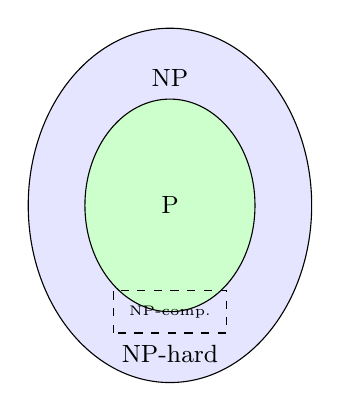
\begin{tikzpicture}[scale=0.9]
      \draw[fill=blue!10] (0,0) ellipse (2cm and 2.5cm);
      \draw[fill=green!20] (0,0) ellipse (1.2cm and 1.5cm);
      \node at (0,0) {\small P};
      \node at (0,1.8) {\small NP};
      \node at (0,-2.1) {\small NP-hard};
      \draw[dashed] (-0.8,-1.8) rectangle (0.8,-1.2) node[midway]{\tiny NP-comp.};
    \end{tikzpicture}
  \end{columns}
\end{frame}

\begin{frame}{The P vs NP Question}
  \begin{alertblock}{The \$1,000,000 Question}
    Does \textbf{P = NP}?\\
    i.e., if a solution can be verified quickly, can it also be \emph{found} quickly?
  \end{alertblock}
  \begin{itemize}
    \item Posed by Stephen Cook in 1971 (Cook's Theorem)
    \item One of the seven \textbf{Millennium Prize Problems}
    \item Most computer scientists believe \textbf{P $\ne$ NP}, but unproven
    \item If P = NP: cryptography breaks, huge scientific impact
    \item \textbf{Practical response:} for NP-hard problems, use approximation algorithms, heuristics, or special-case algorithms
  \end{itemize}
\end{frame}

\begin{frame}{Decidable vs Undecidable Problems}
  \begin{block}{Decidable}
    There exists an algorithm that always terminates and gives the correct yes/no answer.
    Examples: "Is $n$ prime?", "Is this graph connected?"
  \end{block}
  \begin{alertblock}{Undecidable}
    No algorithm can solve this for all inputs.
    \textbf{Halting Problem} (Turing, 1936): "Does program $P$ halt on input $I$?"\\
    \emph{Proof by contradiction} (diagonalisation) shows this is impossible.
  \end{alertblock}
  \begin{block}{Semi-decidable}
    An algorithm exists that halts on YES instances but may run forever on NO instances.
  \end{block}
\end{frame}

\section{Further Reading \& Advanced Topics}
\begin{frame}{Further Reading}
  \begin{itemize}
    \item CLRS 4th ed., Chapter 3 (Asymptotic Notation), Appendix (P/NP)
    \item Scott Aaronson's blog "Shtetl-Optimized" on P vs NP
    \item Complexity Zoo: \url{https://complexityzoo.net/}
    \item 3Blue1Brown YouTube: "P vs NP" (visual intuition)
  \end{itemize}
  \begin{exampleblock}{Recent Developments (2023--2024)}
    \begin{itemize}
      \item New circuit lower bounds pushing toward P $\ne$ NP proofs
      \item Quantum complexity: BQP vs NP relationships clarified
      \item Average-case complexity and fine-grained complexity theory growing rapidly
    \end{itemize}
  \end{exampleblock}
\end{frame}

\begin{frame}{Week 2 Summary}
  \begin{enumerate}
    \item $O(g)$: upper bound; $\Omega(g)$: lower bound; $\Theta(g)$: tight bound
    \item Formal definitions use existential constants $c, n_0$
    \item Proofs: find explicit $c, n_0$; or use limit rules
    \item \textbf{P}: polynomial-time solvable; \textbf{NP}: polynomial-time verifiable
    \item \textbf{NP-complete}: hardest in NP; \textbf{NP-hard}: at least as hard
    \item \textbf{P vs NP}: the central open problem in computer science
    \item \textbf{Halting Problem}: example of an undecidable problem
  \end{enumerate}
  \begin{block}{Next Week}
    Divide and Conquer: Merge Sort, Quick Sort, Recurrence Relations
  \end{block}
\end{frame}
\end{document}
